\section{Problem Formulation and System Boundaries}\label{sec:formulation}
\subsection{From documents to a limited evidence budget}
Let $q$ denote a query and $D$ a collection of parent documents. Preprocessing splits each document into one or more chunks. Dense retrieval scores a parent using its best-matching chunk, which also supplies the representative passage for relevance inference. The distinction matters because judgments apply to parent documents, whereas the model sees bounded passages. A relevant parent does not make every one of its chunks relevant.

Write $\pool_{64}(q)$ for the dense top-64 parents, $\pool_{15}(q)$ for the frozen hybrid shortlist, and $S$ for a selected set of $k=8$ distinct parents. A ranking $\pi(S)$ orders these parents for evaluation. The evidence budget constrains $|S|$ rather than the number of tokens in a generated answer. No answer generator is invoked by the reported retrieval benchmark.

For each candidate $i$, the classical feature pipeline supplies query cosine $c_i$, lexical score $b_i$, a normalized representative vector $v_i$, and cross-encoder logit $z_i$. Define
\begin{equation}
d_{ij}=\min\{1,\max\{0,v_i^\top v_j\}\},\qquad i\ne j.
\label{eq:pair_similarity}
\end{equation}
The set redundancy measure is
\begin{equation}
\red(S)=\frac{1}{\binom{k}{2}}\sum_{\{i,j\}\subset S}d_{ij}.
\label{eq:redundancy}
\end{equation}
This measure lies between zero and one and represents mean clipped cosine, not the percentage of duplicate documents. Negative cosine values are clipped to zero; a zero penalty does not establish that two passages are semantically independent.

The base selector maximizes a relevance--redundancy utility. The refinement instead minimizes redundancy subject to a protected prefix and neural-score conditions. These are different optimization questions. Neither is directly an optimization of the unknown test judgments. Judgments are used only after rankings have been saved, including in the journal's retrospective diagnostics.

\subsection{Candidate opportunity and a recall ceiling}
For a query with nonempty set $J_q$ of positively judged relevant parents and any candidate pool $C$, define judged coverage and a cardinality-aware recall ceiling as
\begin{align}
\operatorname{Cov}(C,q)&=\frac{|C\cap J_q|}{|J_q|},\\
\operatorname{Ceil}_8(C,q)&=\frac{\min\{8,|C\cap J_q|\}}{|J_q|}.
\label{eq:coverage_ceiling}
\end{align}
Every eight-document output drawn from $C$ has Recall@8 no greater than $\operatorname{Ceil}_8(C,q)$. This follows by counting: the output can contain neither more than eight relevant documents nor more relevant documents than the pool contains. Equality is attainable for this diagnostic objective by selecting as many judged-relevant pool members as the budget permits. It is not a claim that a real system can identify them without judgments.

When one pool contains another, both diagnostic quantities are nondecreasing. Candidate expansion can therefore increase the opportunity for judged recall, but it need not increase the recall of a particular selector. Conversely, no optimizer operating only on a fixed pool can recover a relevant parent absent from that pool. This separates three effects that aggregate effectiveness often conflates: corpus-to-pool loss, pool-to-selected-set loss, and ordering within the selected set.

The diagnostic applies to observed judgments. Incompletely judged collections may contain useful unjudged documents, so the resulting ceiling bounds the official judged metric rather than every possible definition of relevance. It also ignores the refinement's prefix and score constraints. An expanded-pool ceiling is thus an optimistic relaxation of the constrained task. The search algorithm alone cannot account for a gap to this ceiling.

\begin{figure*}[t]
\centering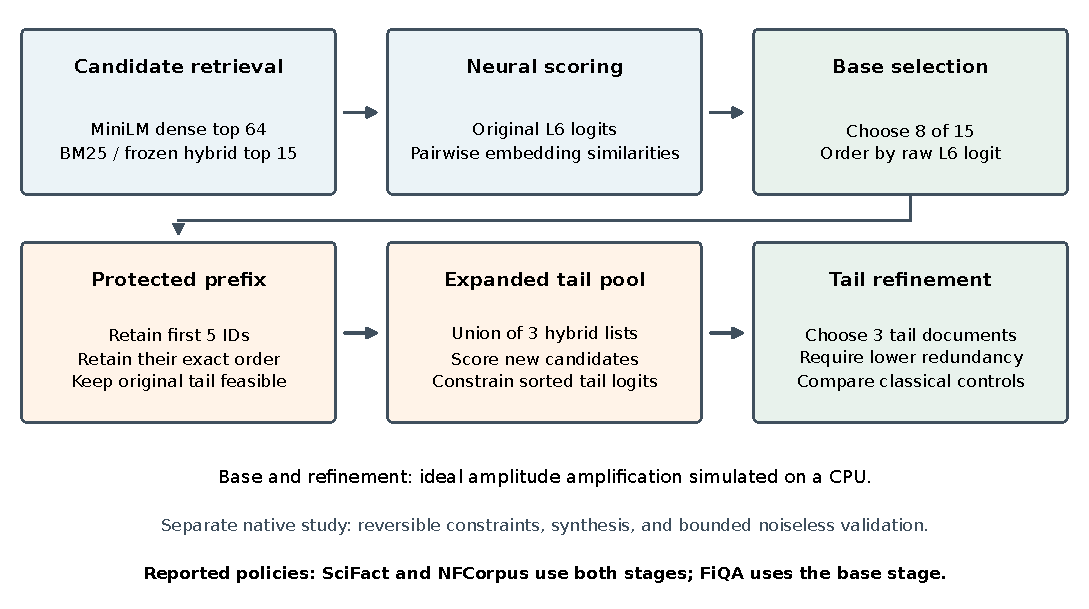
\includegraphics[width=\textwidth]{architecture.pdf}
\caption{System boundaries and reported configurations. Classical retrieval and neural inference precede ideal amplitude amplification simulated on a CPU. The separate native resource study does not replace those classical stages or constitute a full hardware execution of the retrieval pipeline.}
\label{fig:architecture}
\end{figure*}

\subsection{Implementation and measurement boundaries}
Figure~\ref{fig:architecture} distinguishes retrieval, neural relevance inference, base selection, and optional refinement. The application code also supports document ingestion and question-answering interfaces. Their existence does not imply that interface quality, optical character recognition accuracy, or live generated answers were evaluated by these experiments. The measured research pipeline uses public parent-document judgments and frozen passage construction.

The study uses two simulation models. The main selector stores amplitudes for subsets of the required size and constructs their objective values classically. The native study builds reversible circuits with explicit decision and workspace registers. It supplies bounded synthesis and validation evidence; the main selector supplies the retrieval rankings. Neither model includes device routing, noisy execution, or a measured quantum processor.
